% coming soon

We have implemented our switching continual approach in the MAPSIM
environment~\cite{brenner:nebel:jaamas09},
using \system{dlib-ml}~\cite{king:2009} for belief
revision. Sequential sessions use a modified version of Fast
Downward~\cite{fast-downward}, and DT sessions use our own contingent
procedure. We also implemented a simple dual-mode replanning {\em
baseline} approach. Here, when a switching action is scheduled for
execution the DT session executes a single entropy reduction action,
that directly senses an active assumption -- i.e,. We say a fact can
be directly sensed, if there is a DTPDDL {\em sense} declaration that
mentions the fact in its precondition.  Control is then immediately
returned to a new sequential session.


We evaluate our approaches in robot exploration tasks from home and
office environments. Spatially, these consist of {\em rooms}
(office/kitchen/etc), and an underlying topological map that models
smaller areas of space, called {\em places}, and connectivity between
those. The mobile {\em robot} and {\em visual objects} inhabit the
topological space, the latter indicate the category of space they
inhabit -- e.g., Spoons are likely to be in kitchens. By examining
view cones at places for particular objects, the robot is able to: (1)
categorise space at high (room) and low (place) levels, and (2) find
objects for the user, exploiting information about object
co-occurrence and room categories for efficiency. Also, in the
presence of a person, the robot can ask them about the location of
objects. 


We compare our switching planner with the {\em baseline} in several
realistic tasks, with the number of rooms ranging from 3 (12-places,
16-objects, $|$states$|$$>\sim10^{21}$) to 6 (26-places, 21-objects,
$|$states$|$ $>10^{36}$). For or experiments we model three sensors:
{\em Reliable} sensors have a $0.1$ probability of a false negative,
{\em semi-reliable} have a chance of $0.3$ of false negative and $0.1$
of false positive , and finally {\em noisy} sensors with probabilities
of $0.5$ and $0.2$ respectively. Each object class is assigned one
sensor model, so e.g. cornflakes may be harder to detect than
refrigeratos. To determine the influence of the sensor model, we
performed several experiments where we only changed the difficulty of
the target object(s). All non-target objects remain unchanged so the
planner may exploit object co-occurances with reliable objects to
compensate for the increased sensor noise.

We evaluate with DT sessions taking $b_0$ admitting between 20 and 200
abstract states with non-zero probability. We run 50 simulations in
each configuration, and have a timeout on each simulation of 30
minutes (1800 seconds)\footnote{All experiments were conducted on a
  2.3GHz AMD Opteron using one CPU core.}. The continual planning
times are reported in Figure~\ref{fig:results-time}, and the quality
data in Figure~\ref{fig:results-quality}.
%%
For Items~$a$-$e$ the goal is to find objects and report their
position to a user. In some cases there is a non-zero probability that
no plan exists, as the desired object might not be present in the
environment. Item~$f$ reports for tasks requiring indirect sensing,
where the robot must relocate to a room with a particular category
(e.g. kitchen). the {\em baseline} is not able to complete Item~$f$,
so is omitted from that reporting.  Because reward is only allocated
once, on the achievement of the goal,  we find it
intuitive to report average plan costs and the success rates in
problems that admit a solution (i.e., positive reward scaled by a
constant factor).

\begin{figure}[h!]
  % \centering
  % 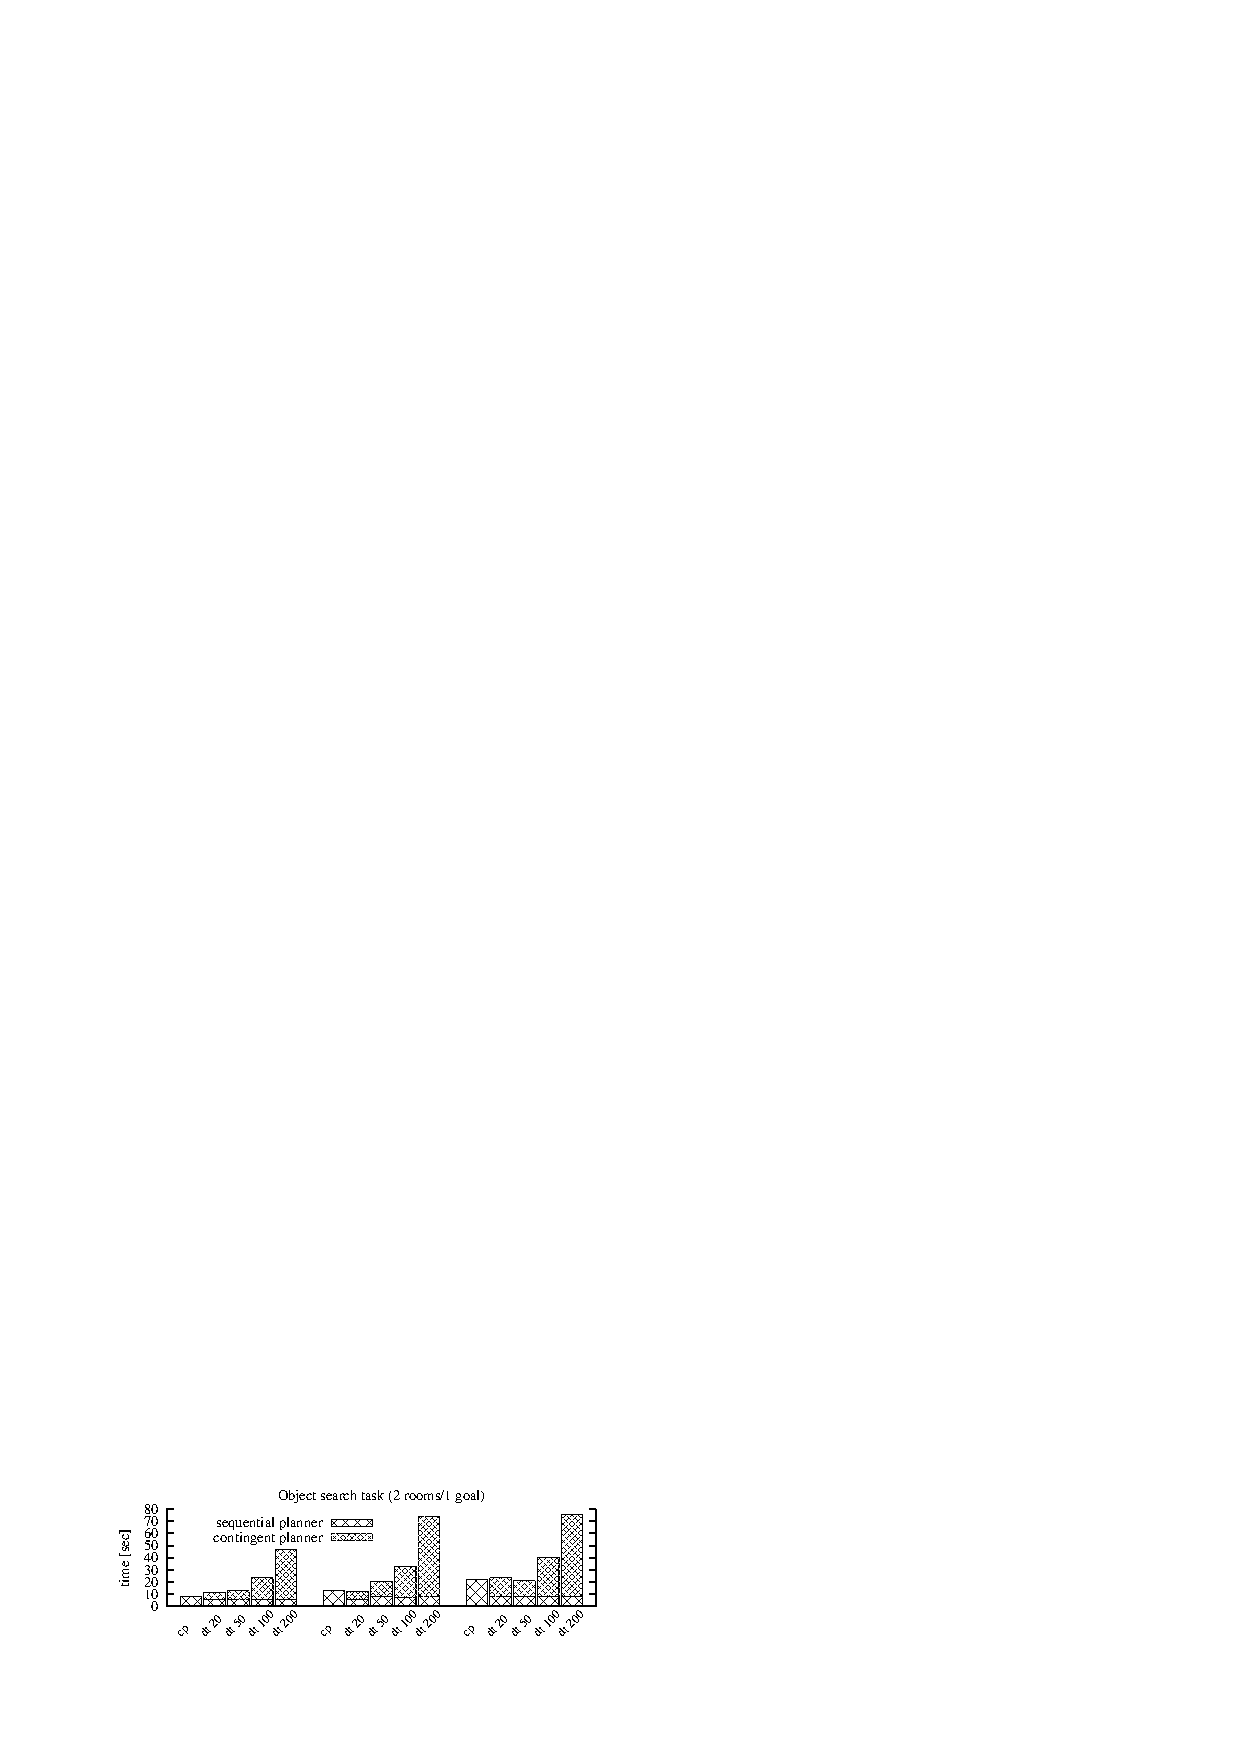
\includegraphics{dora1-time}\hfill
  % \vspace{2mm}
  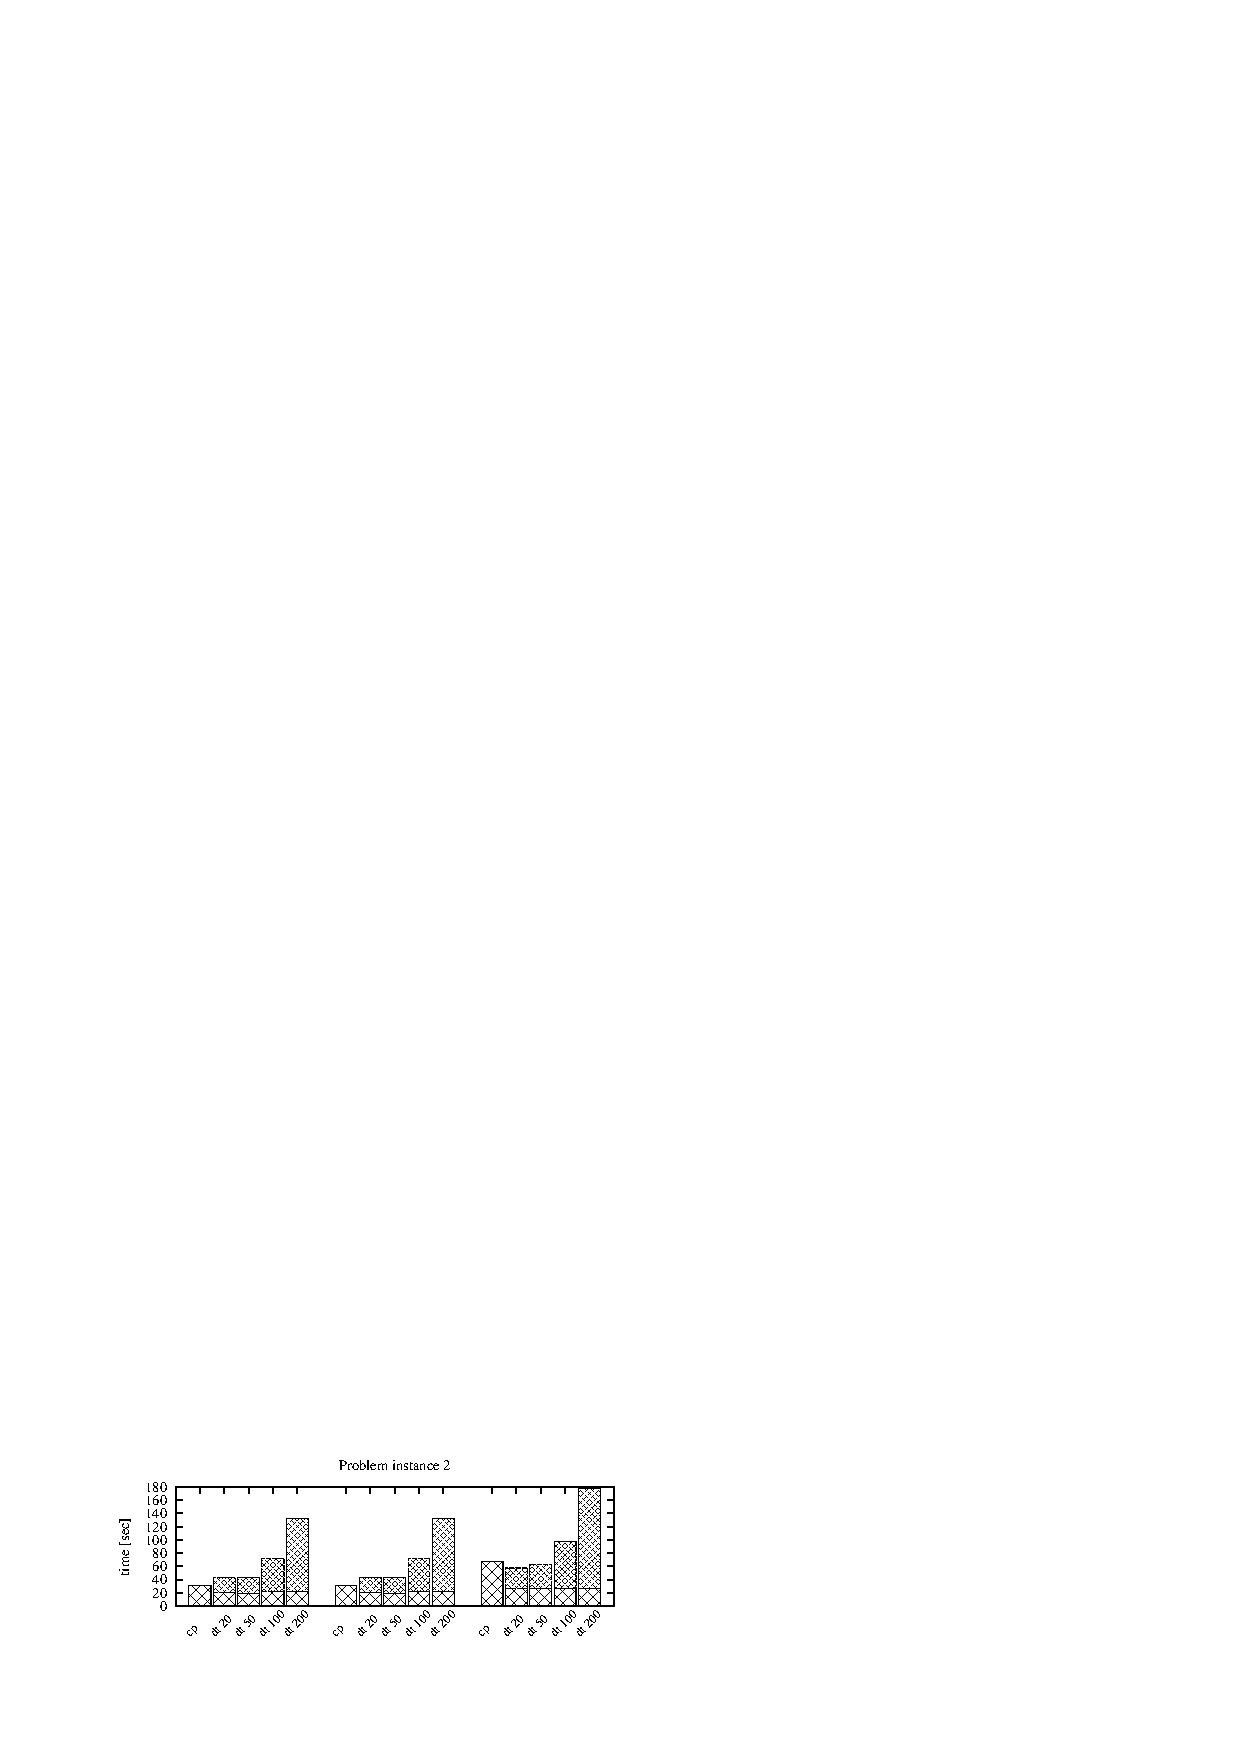
\includegraphics{dora2-time}\hfill
  % \vspace{2mm}
  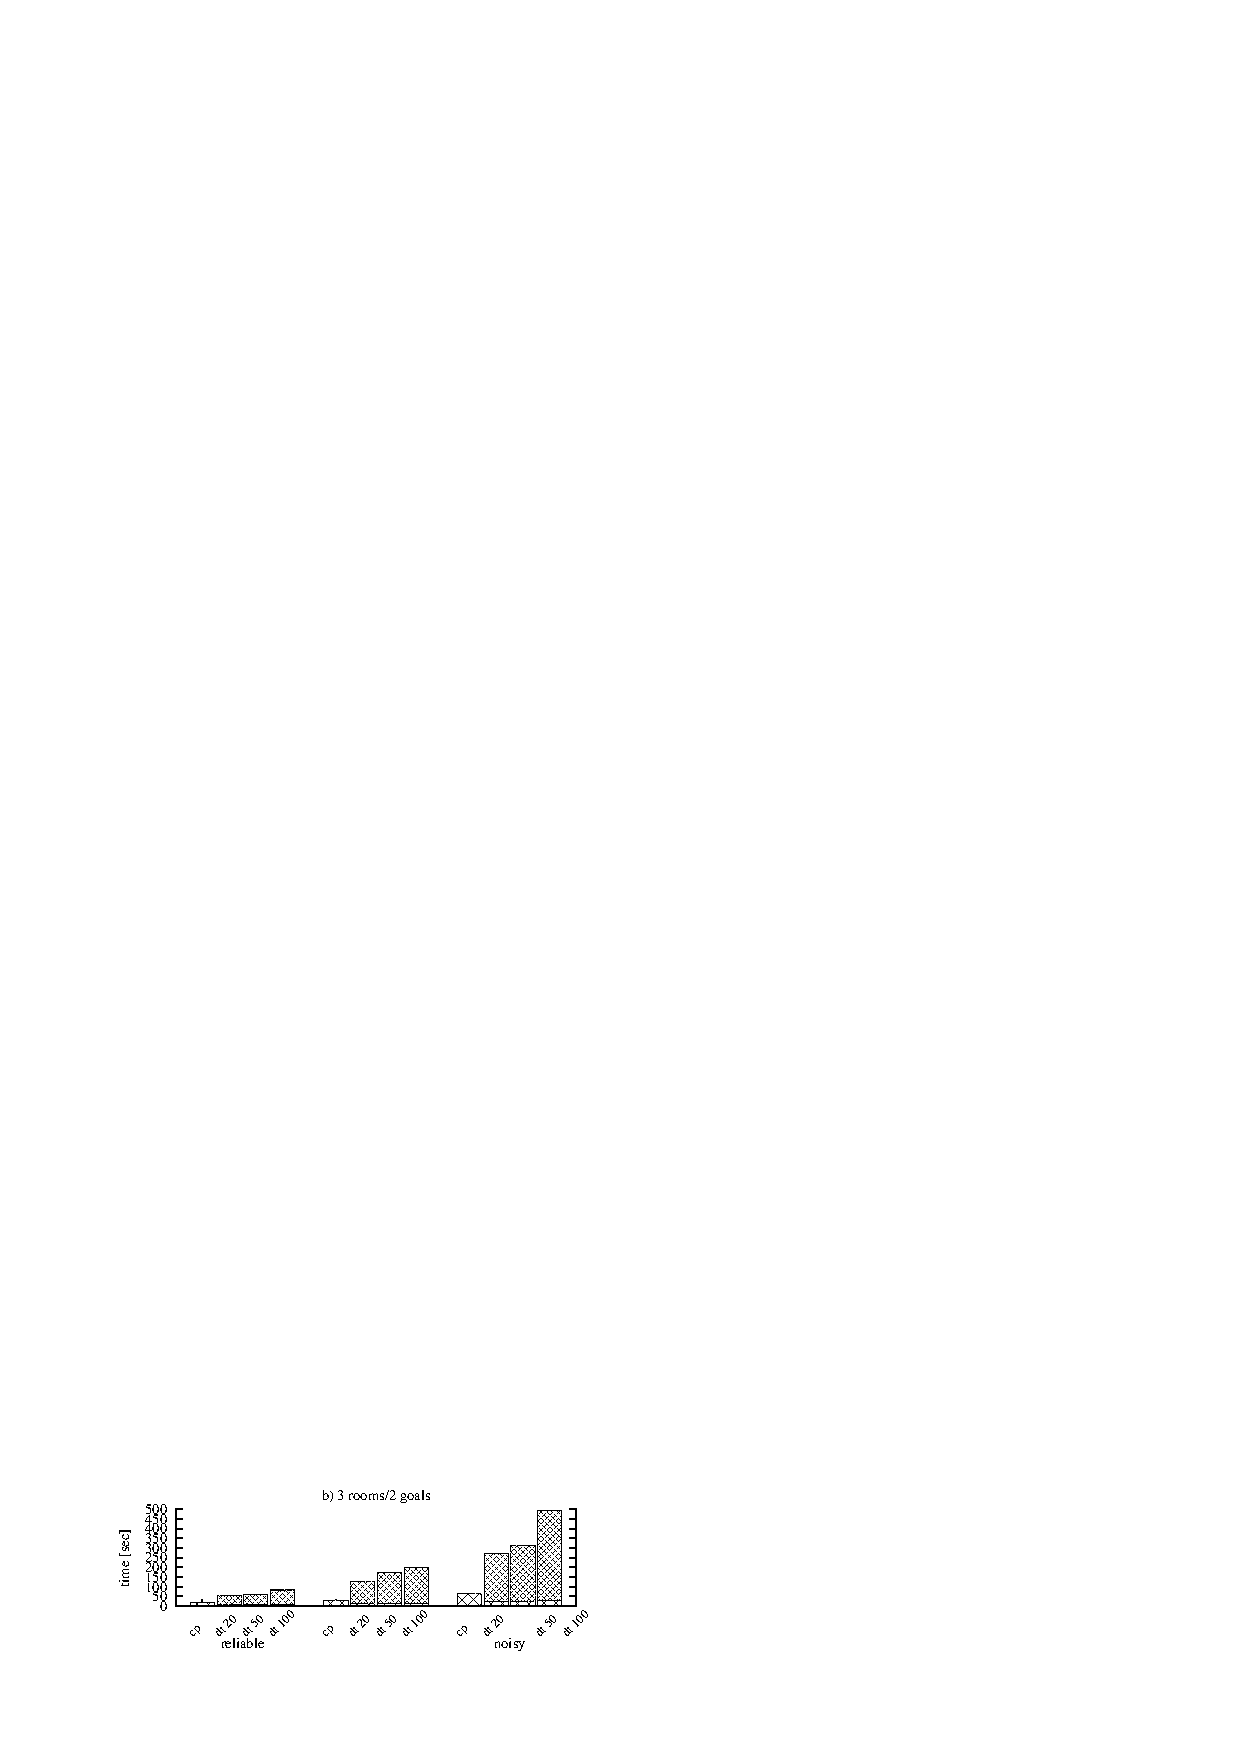
\includegraphics{dora3-time}\hfill
  % \vspace{2mm}
  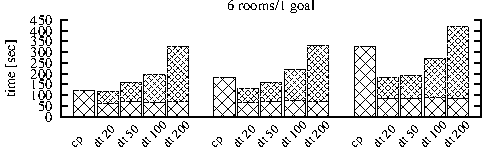
\includegraphics{dora4-time}\hfill
  \vspace{2mm}
  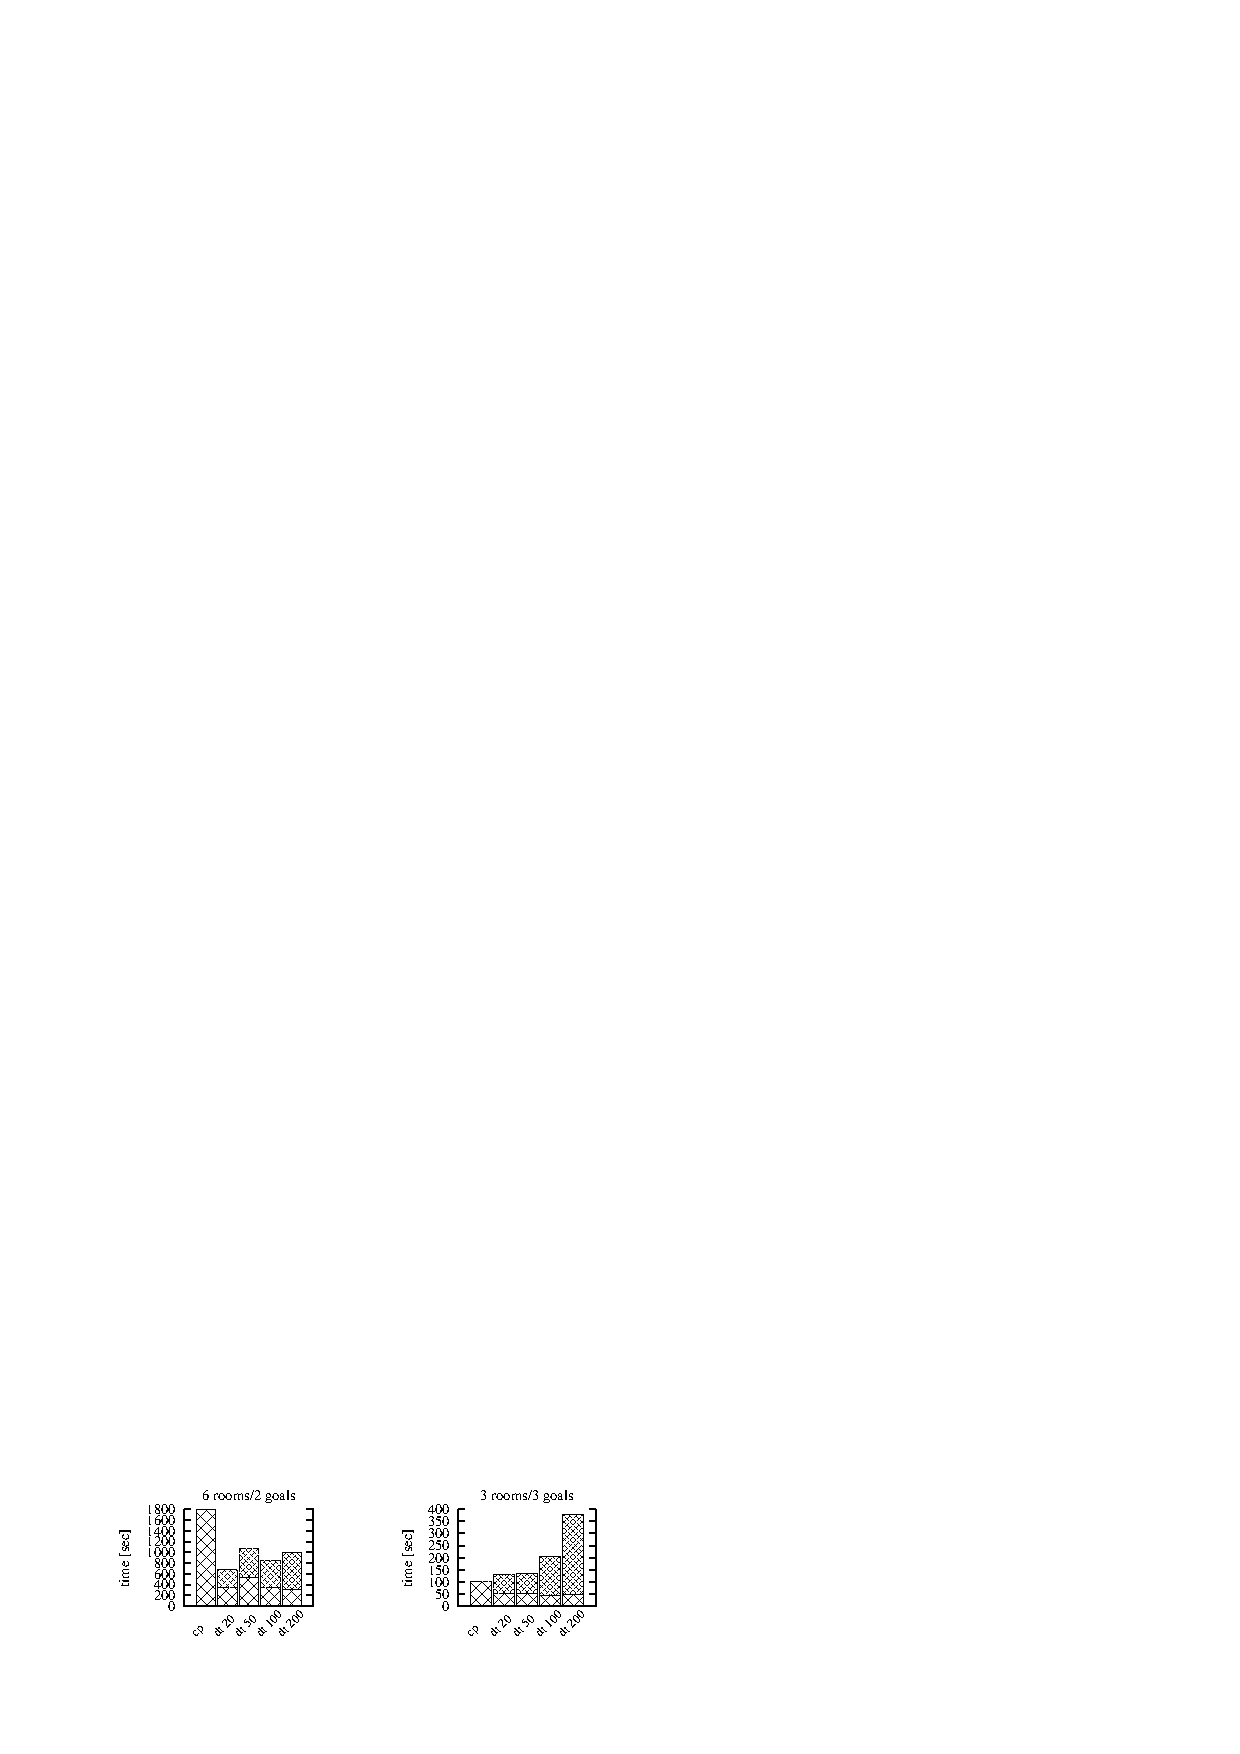
\includegraphics{dora56-time}\hfill
  % \vspace{2mm}
  % 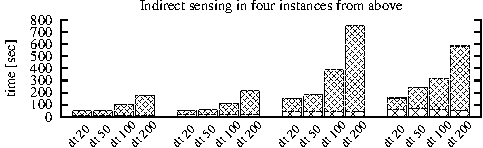
\includegraphics{dora-cat-time}\hfill
  \caption{Average runtime}
  \label{fig:results-time}
\end{figure}

\begin{figure}[h!]
  % \centering
  % 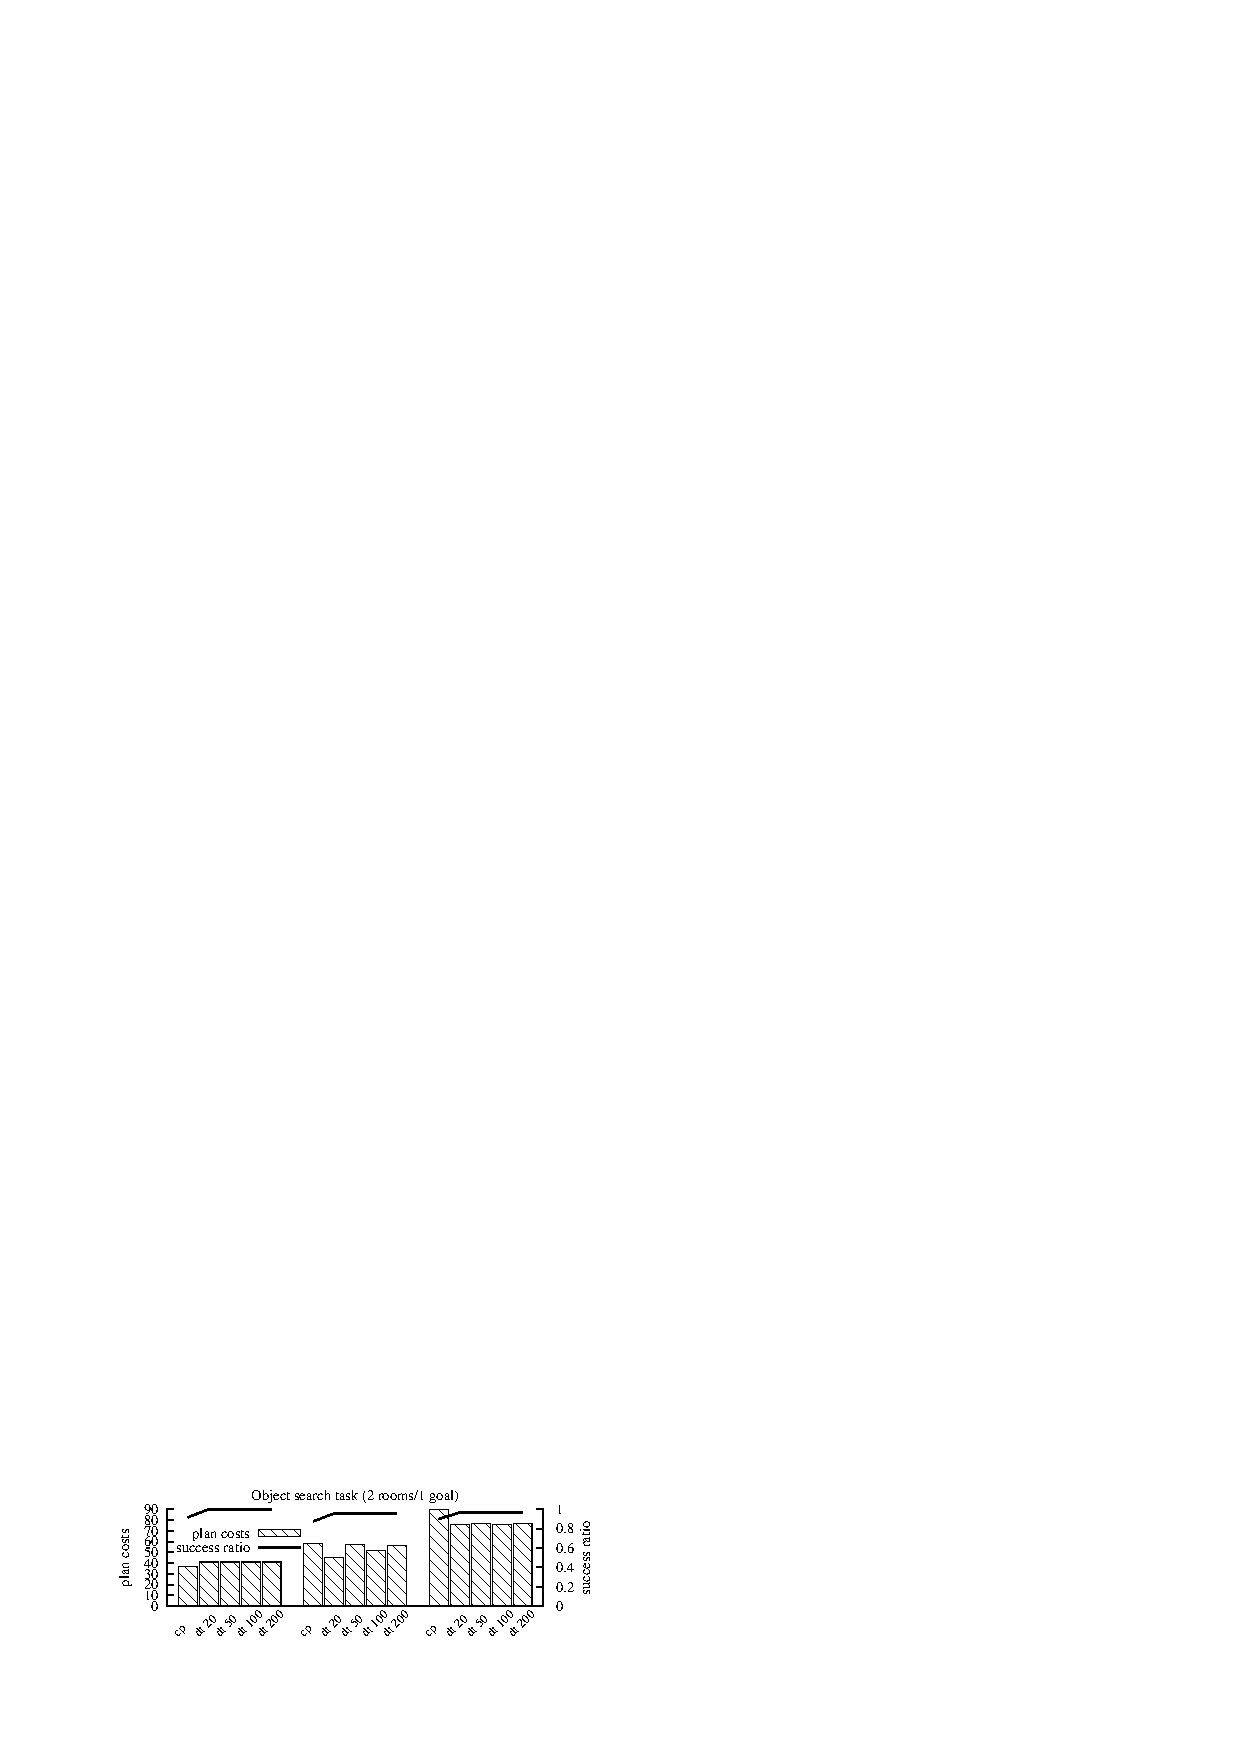
\includegraphics{dora1-quality}\hfill
  % \vspace{2mm}
  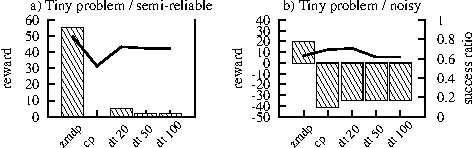
\includegraphics{pomdp-quality}\hfill
  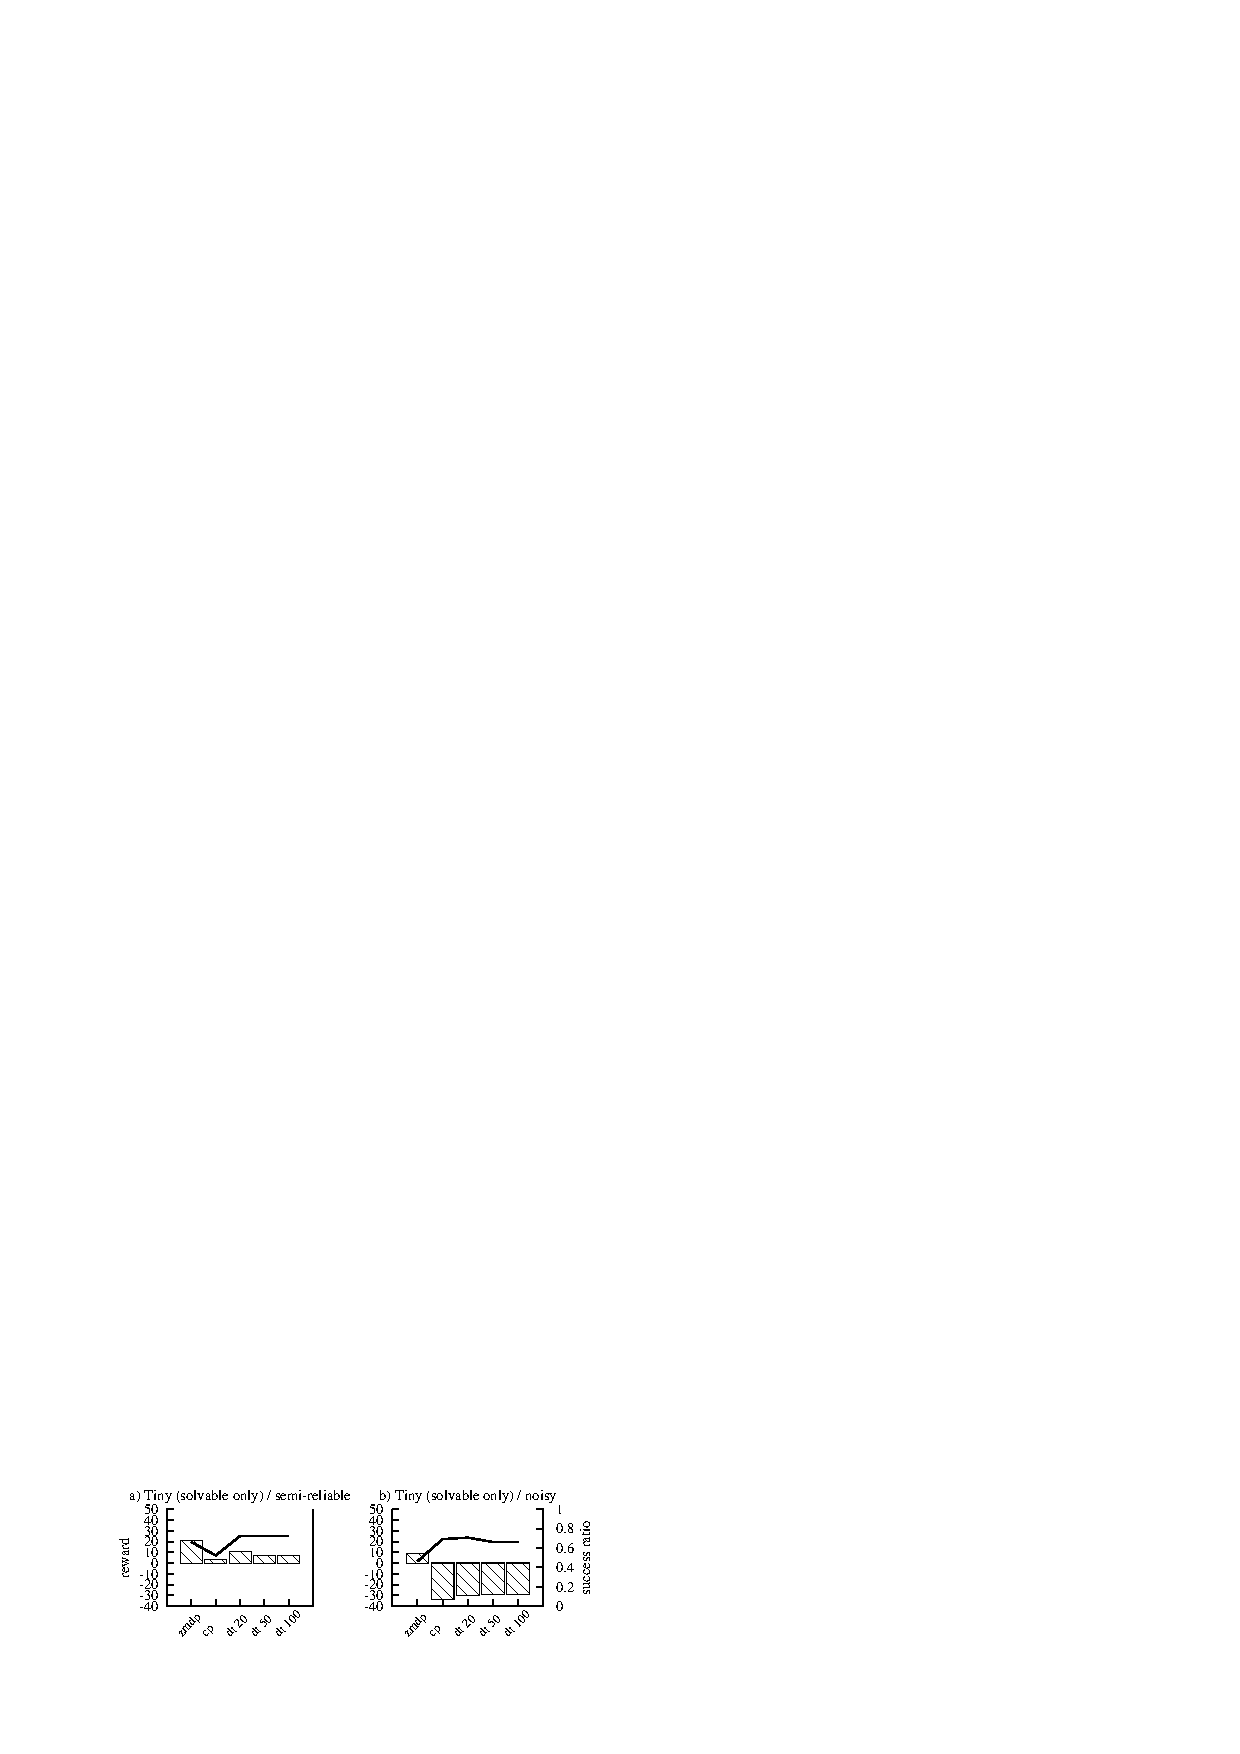
\includegraphics{pomdp-solvable-quality}\hfill
  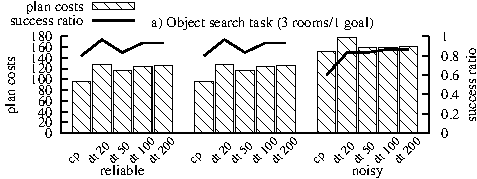
\includegraphics{dora2-quality}\hfill
  % \vspace{2mm}
  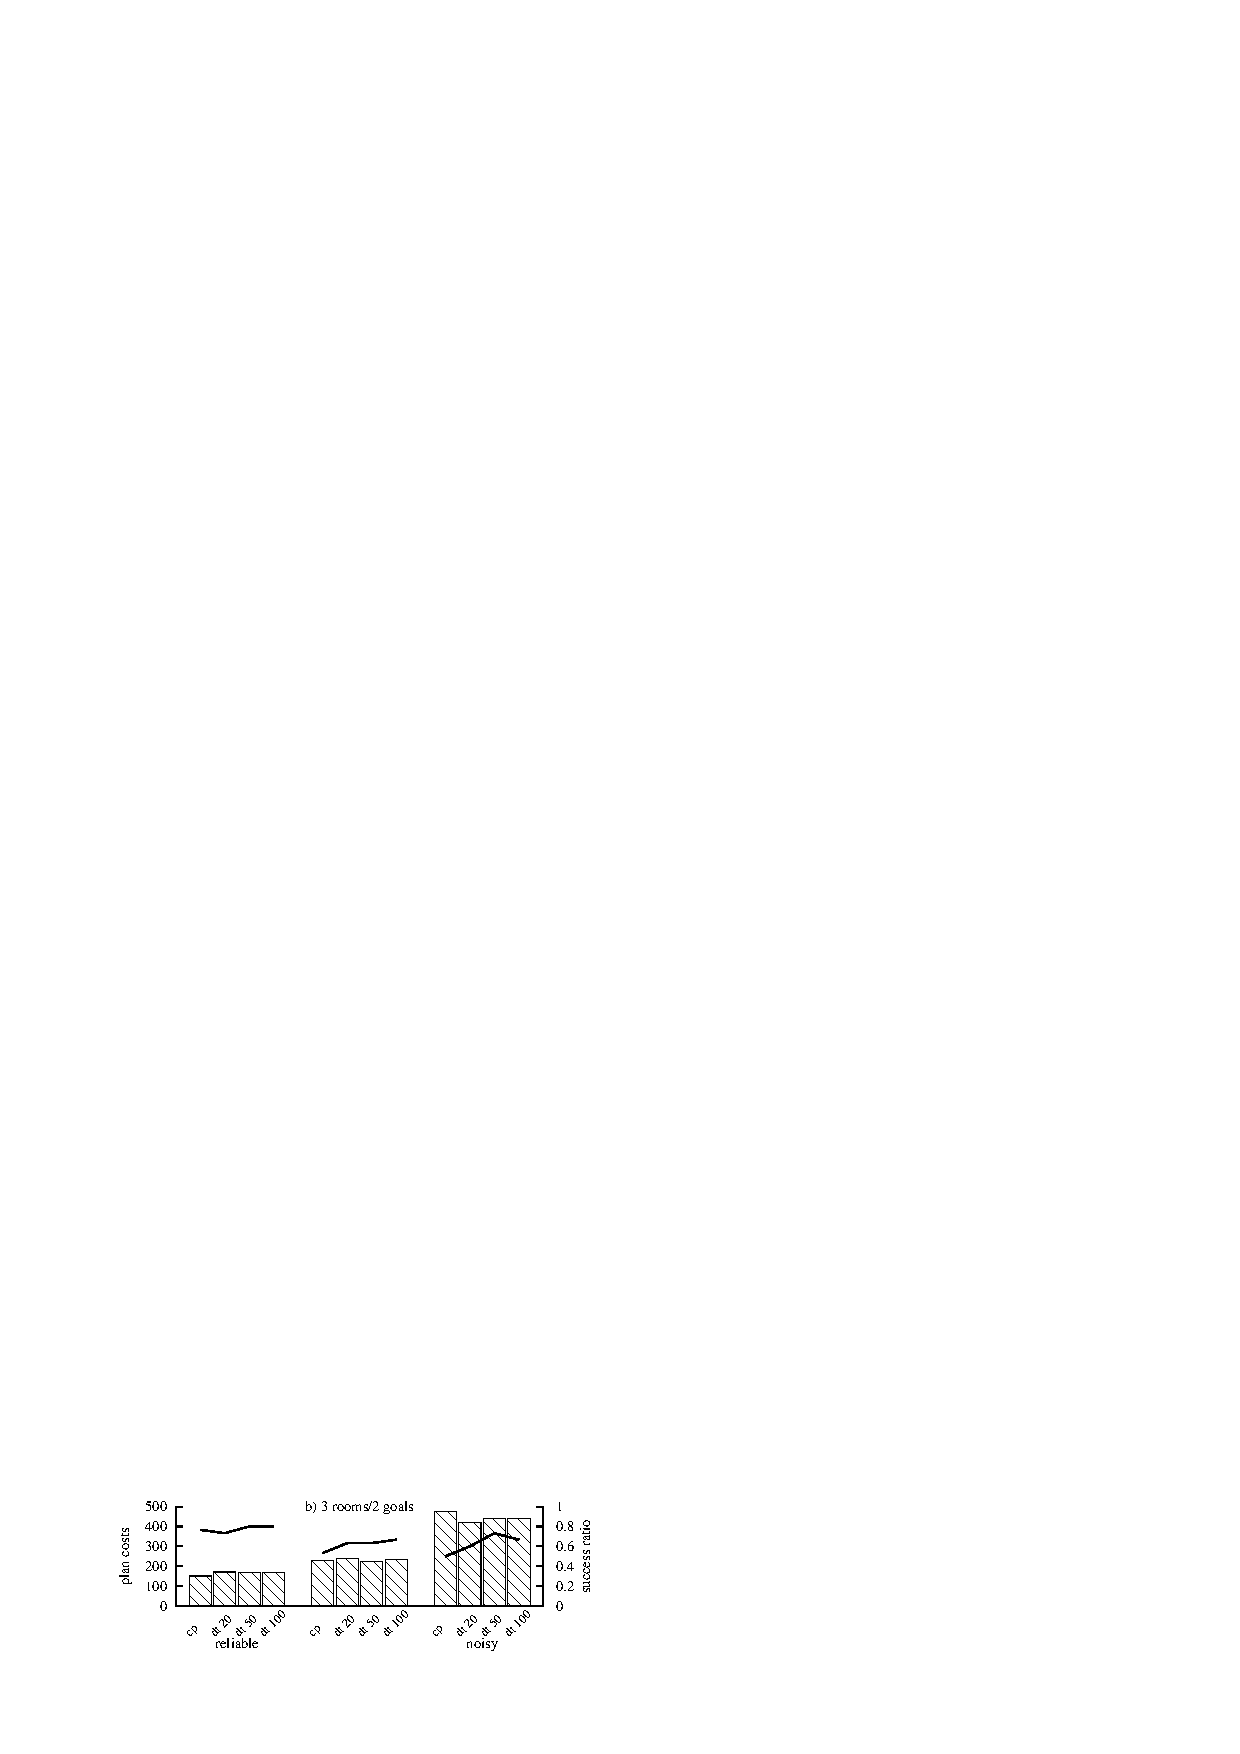
\includegraphics{dora3-quality}\hfill
  % \vspace{2mm}
  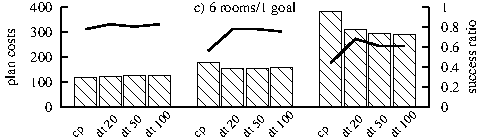
\includegraphics{dora4-quality}\hfill
  \vspace{2mm}
  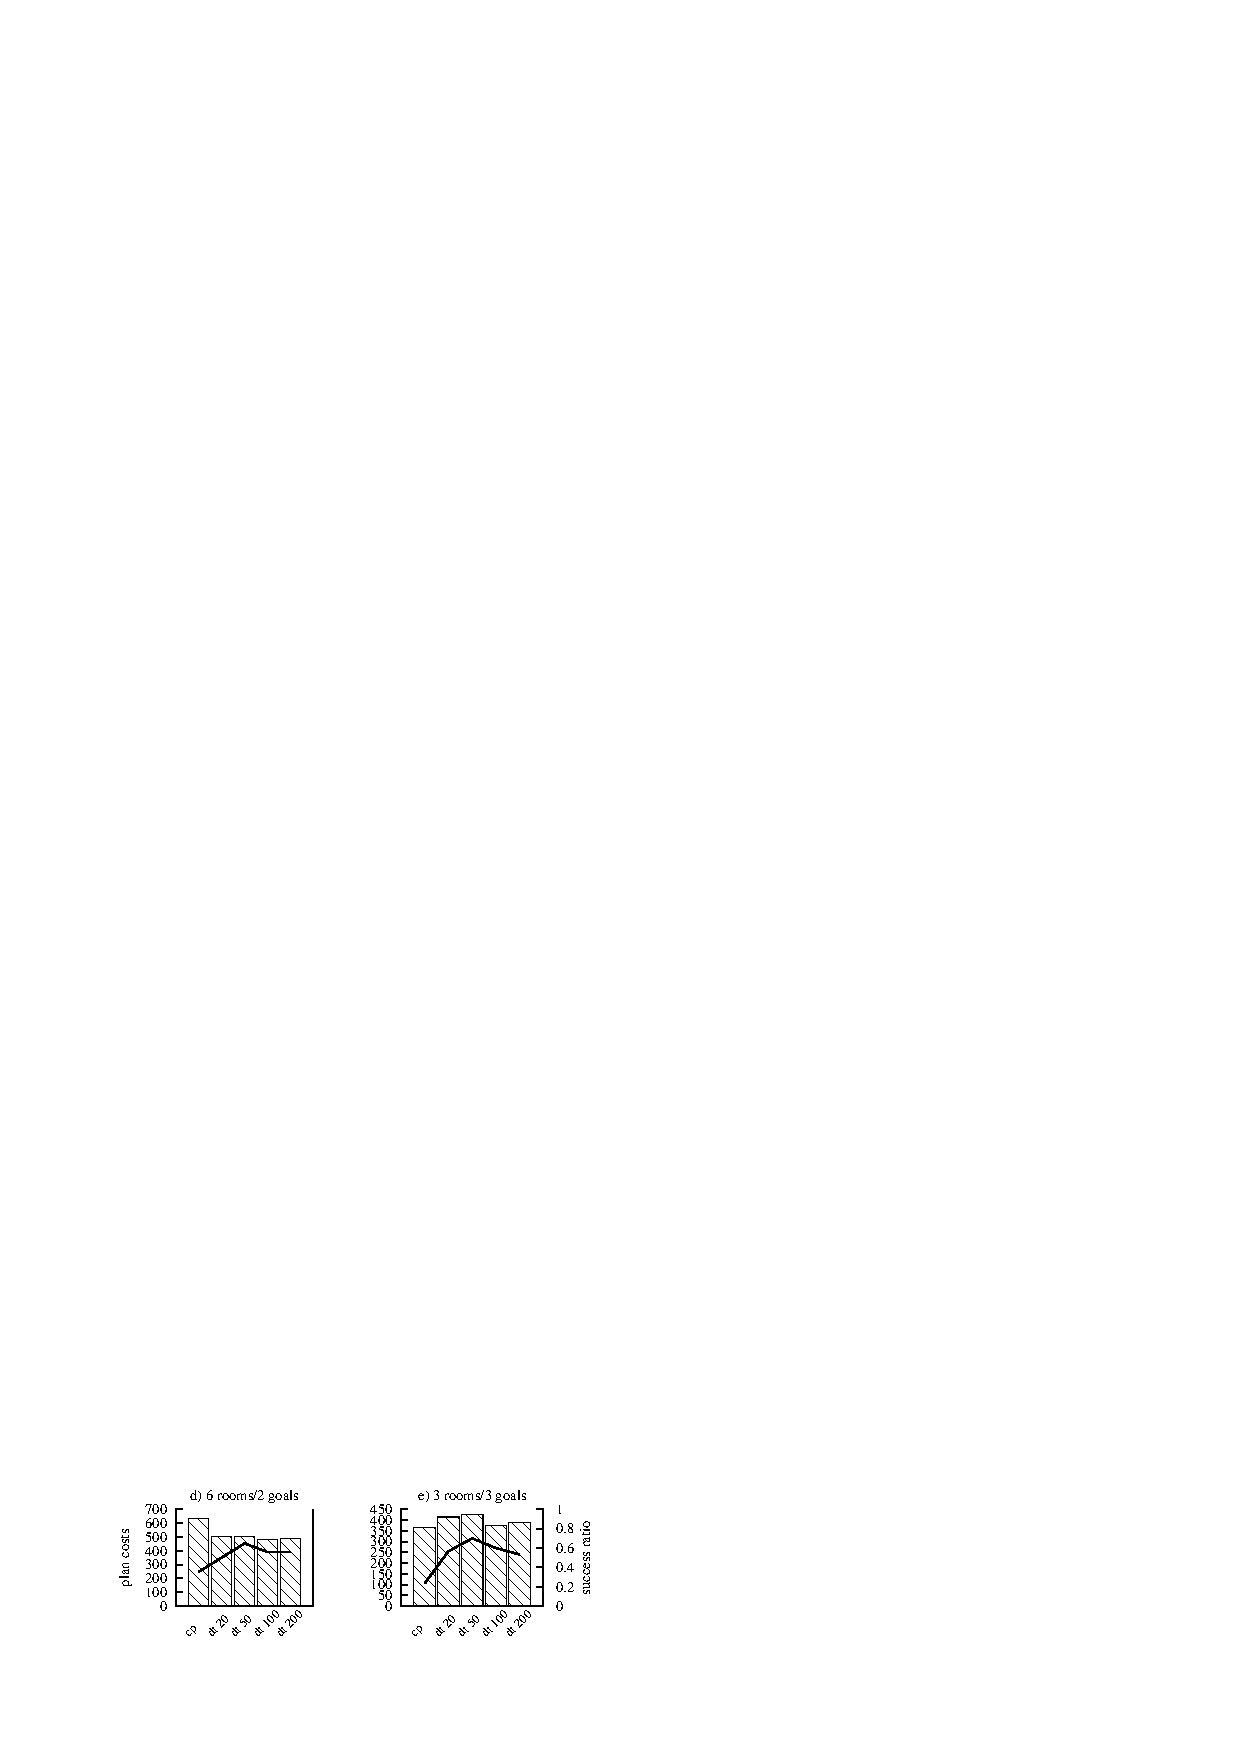
\includegraphics{dora56-quality}\hfill
  % \vspace{2mm}
  % 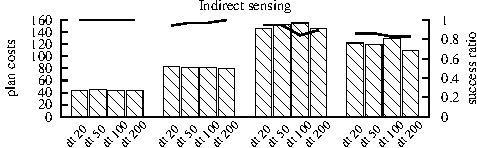
\includegraphics{dora-cat-quality}\hfill
  \caption{Average plan costs and number of successful runs.}
  \label{fig:results-quality}
\end{figure}

We find that if sensing is reliable there is little to be gained
through DT sessions, as the greedy approach of the {\em baseline} is
sufficient. As sensing degrades contingent planning pays off.  Time
spent in DT planning increases steeply as the abstraction $\bstate_0$
becomes more refined.  That refinement seems to be paying off in terms
of the success rate, particularly for tasks $d$ and $e$. For less
refined initial configurations, the increased cost of DT
planning is compensated for by a decrease in Fast Downward planning
times. The relatively high success rate irrespective of the level of
refinement in the initial configuration indicates the effectiveness of
using conditional entropy to guide abstraction refinement in our
setting.

%%% Local Variables: 
%%% mode: latex
%%% TeX-master: "aaai11"
%%% End: 
